\documentclass[12pt,a4paper, notitlepage]{article}
\usepackage{graphicx}
\usepackage{setspace}%for double spacing etc
\usepackage[top=1.0in, bottom=1.0in, left=1.5in, right=1.0in, twoside]{geometry}
%\usepackage[latin1]{inputenc}
\usepackage{amsmath}
\usepackage{amsfonts}
\usepackage{amssymb}
\usepackage{bm}
\usepackage{graphicx}
\usepackage{caption}
\usepackage[T1]{fontenc}
\onehalfspacing
\begin{document}
	\begin{singlespace}
		\begin{center}
\vspace*{20pt}
\begin{LARGE}
%\textbf{Vision based Techniques of Identification for Robotic Systems and its Applications}\\
\textbf{DESIGN AND CONTROL OF A TELE-OPERATED MOBILE PLATFORM}\\
\end{LARGE}
\vspace*{60pt}
\begin{Large}
Synopsis of the doctoral dissertation\\
~\\
~\\
~\\
by\\
\end{Large}
\vspace*{50pt}
\begin{large}
\textbf{Amaren Prasanna Das}\\
(2011MEZ8364)\\
\end{large}
\vspace*{40pt}
\begin{figure}[h]
\centering
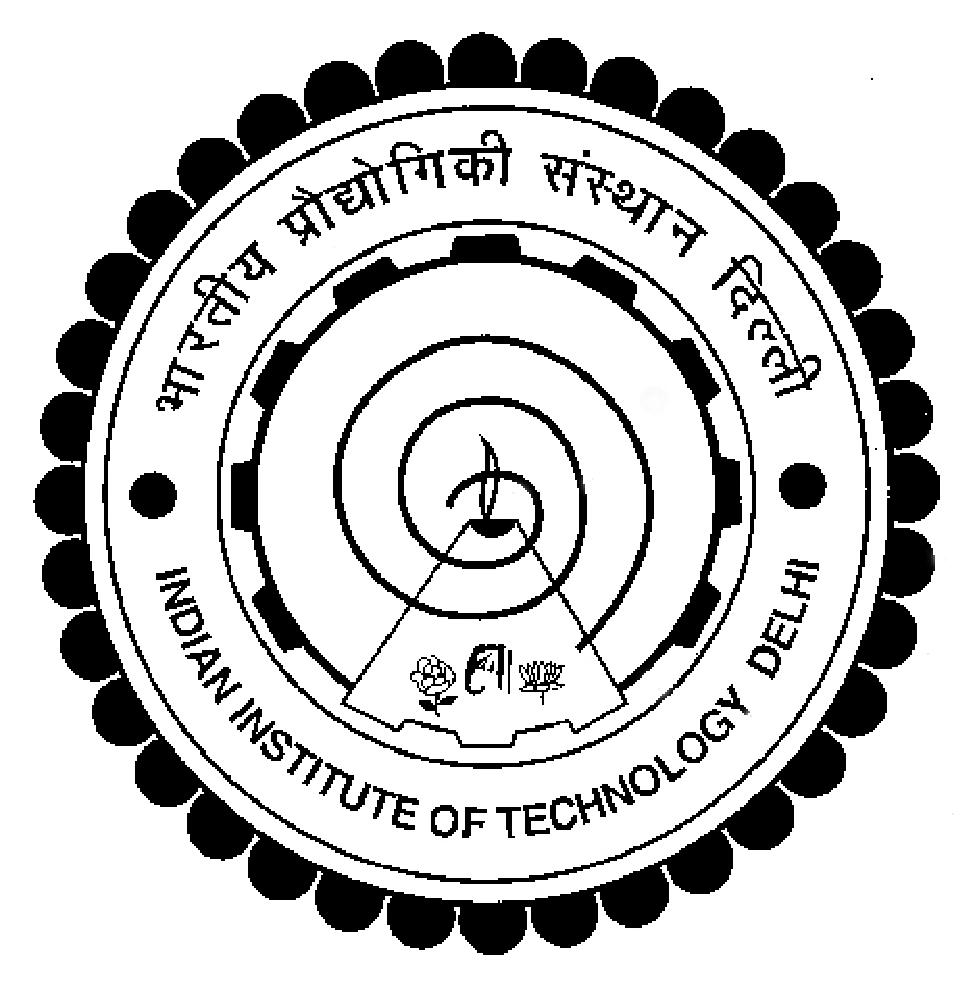
\includegraphics[scale=0.3]{fig/iitlogo.eps}
\label{iitd}
\end{figure}
\vspace*{40pt}
\begin{Large}
Mechanical Engineering Department\\
Indian Institute of Technology Delhi\\
Hauz Khas, New Delhi-110016\\
\end{Large}
\vspace*{10pt}
November 2018
\end{center}
\thispagestyle{empty}
\newpage
\thispagestyle{empty}
	\end{singlespace}
	~\\
	\newpage
	\section{Introduction}
	The use of mobile robots is growing in numerous	applications such as planetary exploration, police operations, e.g.,rescue \cite{guarnieri2004development},	explosive ordnance disposal, military operations \cite{pal2007mobile} e.g., reconnaissance	missions, surveillance, and neutralization of improvised explosive device, hazardous site exploration, and more. Similar requirements exist for inhospitable environmental conditions existing in chemical, space \cite{sheridan} or nuclear industries \cite{briones1994wall},\cite{kim20173d} and \cite{ohno2011robotic}.   Teleoperated mobile robots   are suitable for these applications  as the work space required to be covered is very large and it is essential to maintain  physical separation between the robot and its control station. Moreover the remote environment is in general unknown.
	
	 This research  was motivated by a similar requirement for in-situ measurement and mapping  of the radioactive radiation, mostly neutron field, inside the vault and cave areas of   K-130,  K-500,  and Medical Cyclotron operational at VECC, Kolkata, West Bengal.  Radiation mapping of these areas are  mandatory requirements for getting safety clearance from regulators during  commissioning of new units and at regular intervals during operational life of the cyclotron facility. 
	 
	 A four wheeled tele-operated mobile robot with a manipulator was designed for the above requirement. The 3D model and the actual system are shown in Figures \ref{fig:robo3Dmodel} and \ref{fig:roboActual}, respectively. The manipulator is a vertically moving scissor mechanism with the radiation detector mounted on the top for vertical scanning. This  mobile robot is to be teleoperated over a wireless network. Design of the mobile robot  is customized to the environment and mission requirements. The vehicle is equipped with an on-board camera which continuously streams video to the control station. A human operator based on  this video feedback controls the movement of the mobile robot and the manipulator. Radiation  and odometer data are also relayed back to the operator station for real-time radiation mapping. 
	 
	  \begin{figure}[ht]
	 	\centering
	 	
	 		\centering
	 		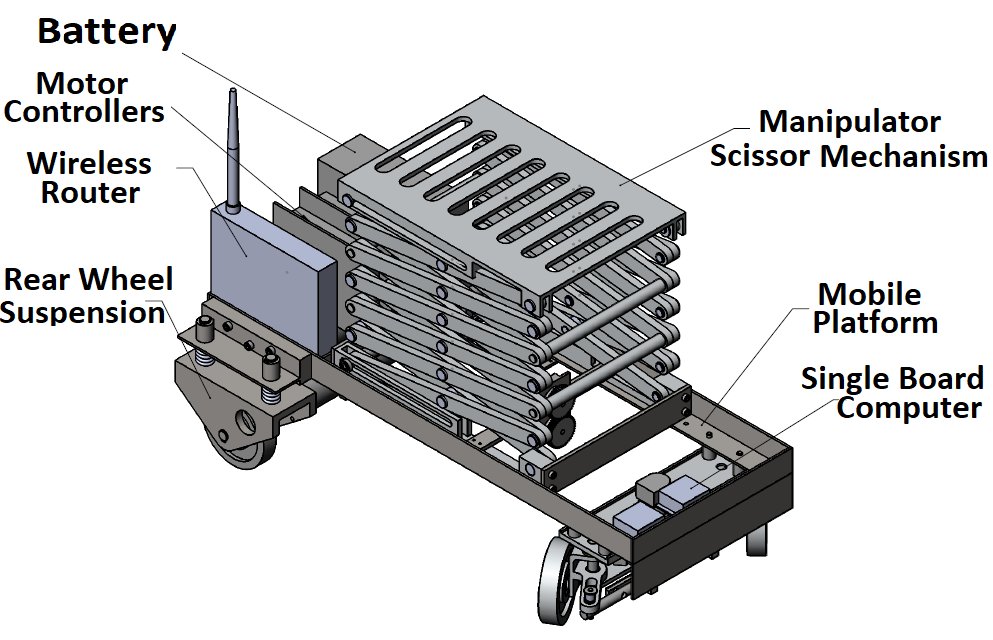
\includegraphics[width=.8\textwidth,keepaspectratio]{fig/robo3Dmodel}
	 		\captionof{figure}{3-D Model of the mobile manipulator}
	 		\label{fig:robo3Dmodel}
	 \end {figure}
 
	 	\begin{figure}
	 		\centering
	 		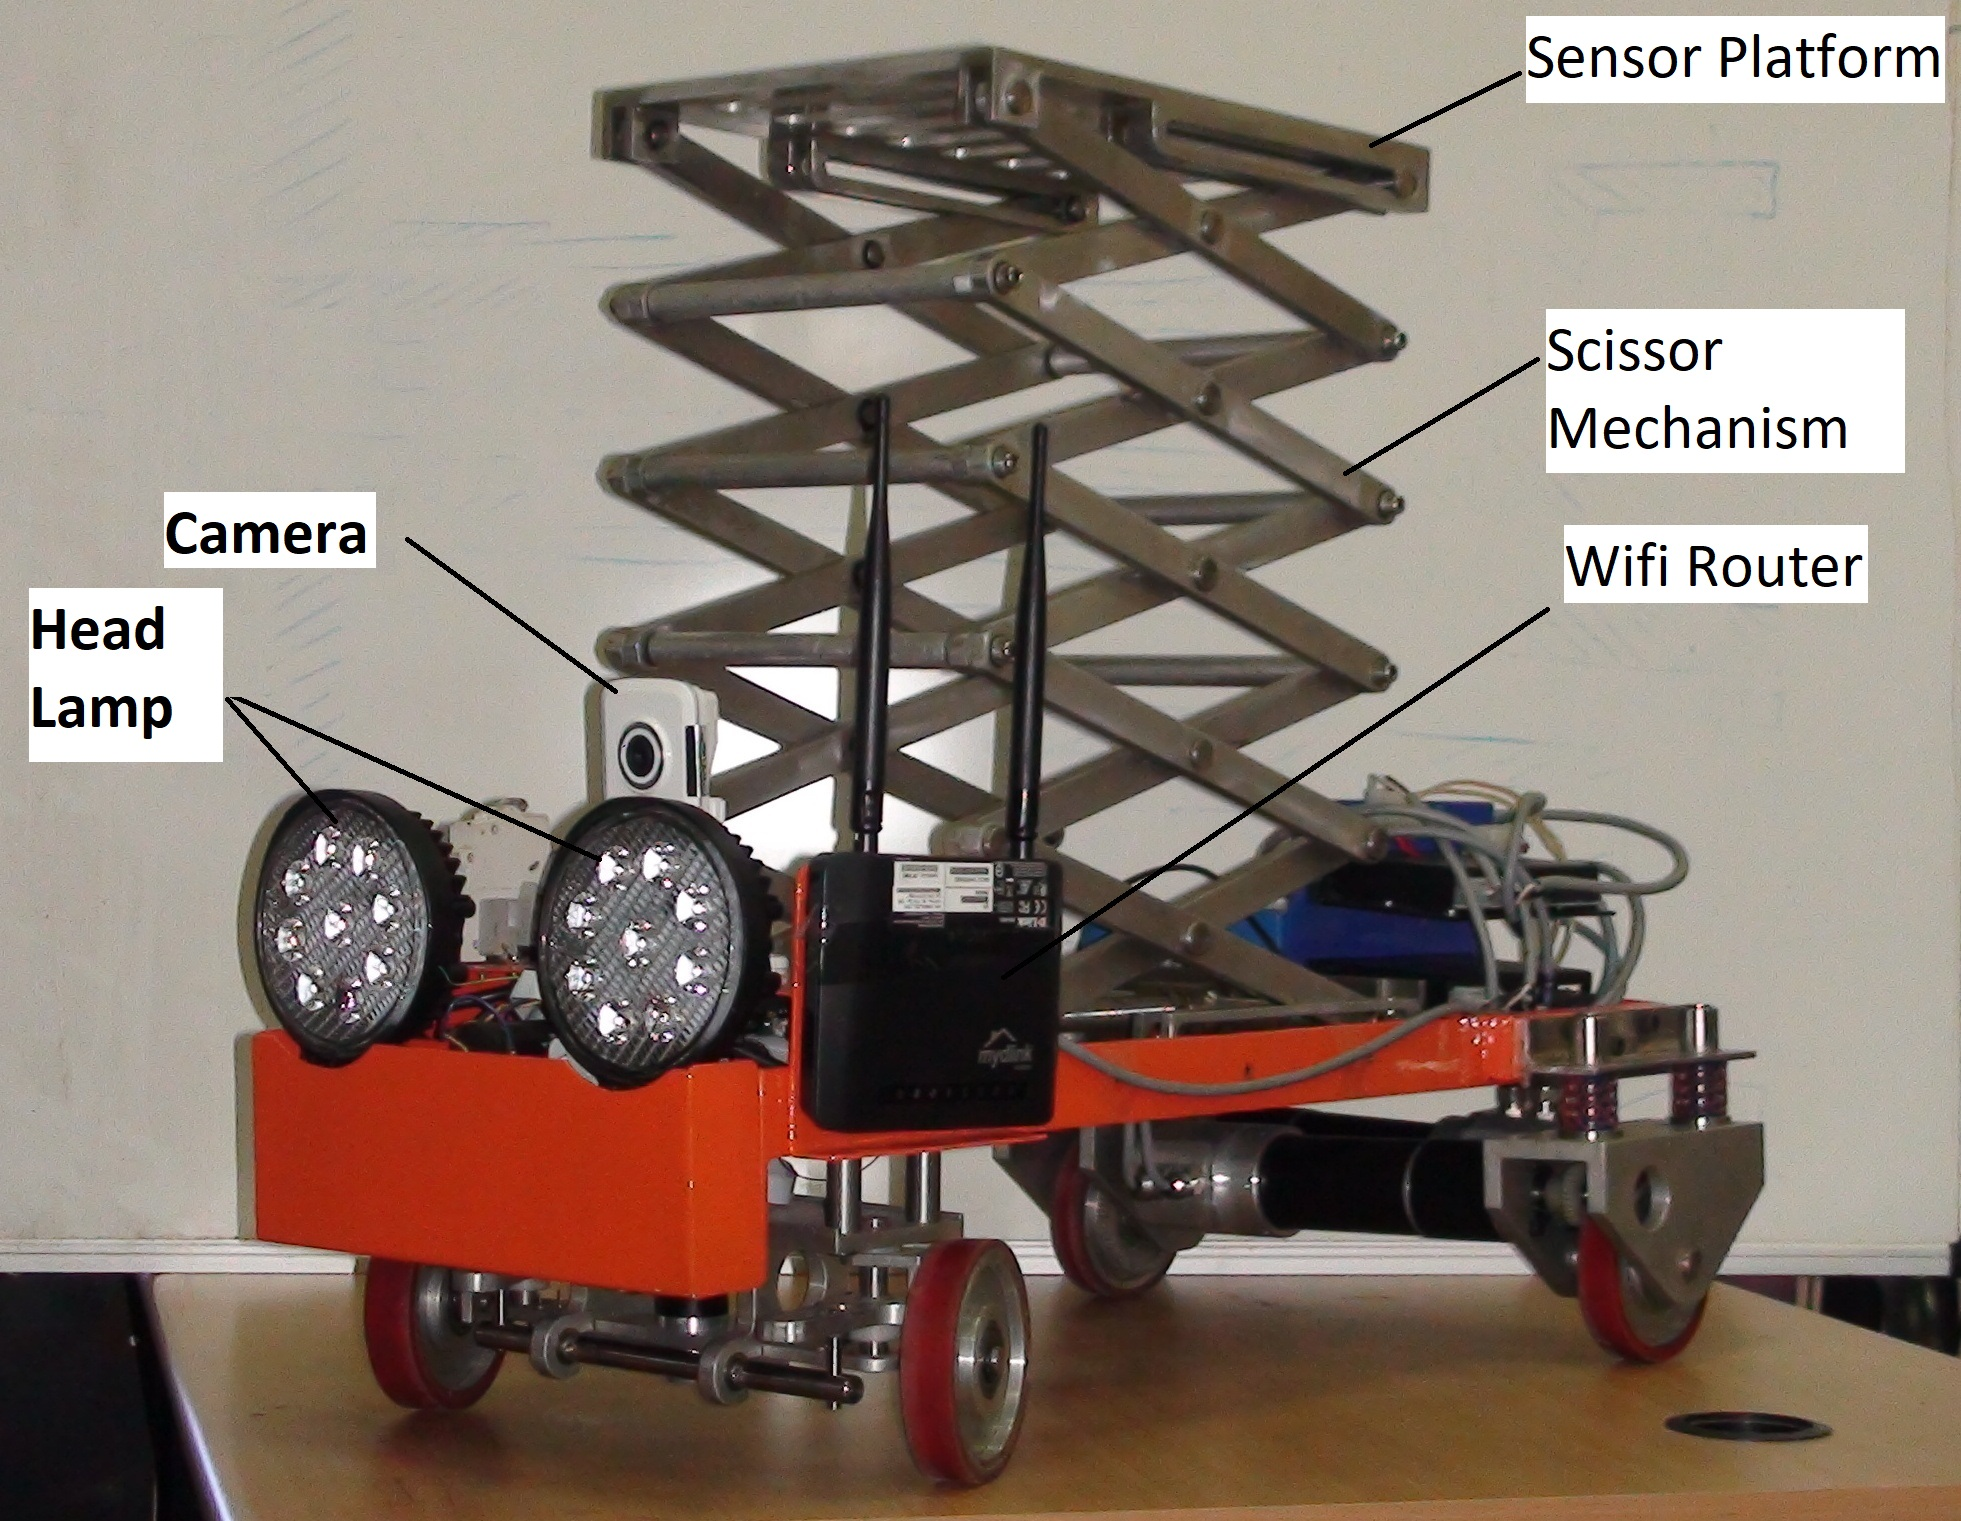
\includegraphics[width=.7\textwidth,keepaspectratio]{fig/roboActualN}
	 		\captionof{figure}{Photograph of the actual system}
	 		\label{fig:roboActual}
	 	\end{figure}
	 
	 
	    
	%\subsection{Thesis Objectives}


	\subsection{Contribution of the Thesis}
		The original contributions of the present research are listed below:
	\begin{enumerate}	
		\item Design of a customized teleoperated mobile robot for remote surveillance and mapping application.
		\item Development of kinematic and dynamic model of the robot at hand.
		\item Control architecture required for intuitive teleoperation of this mobile robot.
		\item Predictive visual feedback control to alleviate problem arising due to time delayed.		
	\end{enumerate}
\subsection{Thesis Organization}
The thesis will have following chapters as listed below.
\begin{itemize}
\item [ ] {Chapter 1: Introduction}
\item [ ] {Chapter 2: Literature Review}
\item []{Chapter 3: Design of a Mobile Robot}  
\item []{Chapter 4: Mathematical Modelling of Wheeled Mobile Robots }
\item []{Chapter 5:Control of mobile manipulator }   
\item []{Chapter 6: Simulation of Tele-operation }
\item []{Chapter 7: Predictive Display }
\item []{Chapter 8: Conclusions}
\item []{Bibliography}
\end{itemize}
	%\section{Literature Review}
%	Literature  survey was carried out in different fields such as use of teleoperated  mobile robots in space \cite{sheridan}, underwater  \cite{sheridan1978human} and nuclear field such wall climbing robot \cite{briones1994wall},\cite{galt1997tele}
	%\subsection{Use of robot in nuclear industries }
	\section{Design of a Mobile Robot}
	\label{Design}
	Most of the mobile robots presented in literature uses differential wheel drive  with passive castor, as in \cite{yamamoto1992coordinating}, \cite{rajendran2004} and \cite{saha1989kinematics}. The other  common methods for locomotion of mobile robots are the omnidirectional wheels  \cite{pin1994new} and \cite{salih2006designing}, and tracked wheel system \cite{suthakorn2009design} and \cite{guarnieri2004development}. According  to  Nagatani \cite{nagatani2000improvement},  a  vehicle  with  Mecanum  wheels  is  susceptible  to slippage and same is the case for tracked vehicle, which are inherently skid steered. The slippage of  wheels prevents  popular dead-reckoning method using rotary shaft  encoders   from  being  performed  well.  Skid steering is not energy efficient, which reduces  mission time for a given power pack, e.g batteries. The major issue with caster supported differential drive robots is that  the castor wheels get stuck even in case of small obstacles less than the $\frac{1}{4}^{th}$ the wheel diameter. 
	
	Based on the above observations, a mobile robot was designed with four wheels which provide better stability. The two rear wheels are driven by independent motors and the front wheels are steered by a single motor through Davis mechanism \cite{TOMBook}. A scissor based vertical lifting platform was mounted on the mobile robot to give the required vertical coverage to the radiation detector. Table \ref{tb:specifications} lists the  specifications of this robot. The key to overall design was to make it light weight, energy efficient, and robust to single actuator failure. Use of positively steered Davis mechanism eliminated the problem associated with castor wheel. Moreover, it satisfies rolling condition of all four wheels for the complete range of steer angle, providing better efficiency. The use of independently driven rear wheels along with the steered front  wheels makes the system over actuated. This is advantageous in case of failure of one actuator. The vehicle can still be driven to a safe location. Independent drive to the rear wheels also eliminates the problem of robot getting stuck up in case  one of the rear wheels looses traction as power can be directed to the other rear wheel. This in contrast to the mechanical differentials drives commonly found in commercial vehicles.  The motor ratings were based on the requirement to ascend and descend a ramp of $15^o$ with 5 Kg pay load. The material of construction is AL6061 to make it light weight.
	\begin{table}[!htbp]
		\caption{Specifications of the mobile manipulator.}
		\label{tb:specifications}
		\centering
		\begin{tabular}{l l l}
			\hline
			
			%\emph{Parameter}  & \emph{Example} & \emph{Font size and style} \\
			%\hline
			Weight  & 70 Kg & Without payload \\ 
			Payload & 10 Kg &---\\
			Footprint & 700 mm $\times$  400 mm & --- \\
			Height Collapsed & 500 mm  & Along  Z-Axis\\
			Height Extended & 1500 mm & Along  Z-Axis  \\
			Steering mechanism & Davis Steering & ---\\
			Turning radius & 415 mm & --- \\
			Ground clarence & 45 mm & ---\\
			Maximum traction speed & 2 m/min & On flat terrain \\
			Ramp climb angle & $30^\circ $ & Checkerboard surface\\
			\hline
		\end{tabular}
	\end{table}
	
	\section{Dynamics of the Wheeled Mobile Robot (WMR)}
	Dynamic model of the mobile robot discussed in Section \ref{Design} is required for verification of its actuator ratings, design of model based controller, and to study the  behaviour under time delay associated with the teleoperation.	 Different methods have  been adopted to derive the dynamic model of WMRs. A general dynamical model was derived for three-wheeled mobile robots with nonholonomic constraints  by B. d'Andrea-Novel \cite{d1991modelling} using  Lagrange formulation.	Alternatively, Thanjavur and Rajagopalan \cite{thanjavur1997ease} have used Kane's method. The  Natural Orthogonal Compliment (NOC) method was used by  Saha et al. \cite{saha1991dynamics}, \cite{saha1989kinematics}  to arrive at the dynamic model. This method has the advantage of inherently taking non-holonomic constraint into consideration. This is matrix based, which makes it easy for numerical simulation.  Simulation  with the actual parameters of the custom designed robot was done for  motion over a circular ramp with inclination $15^o$ and radius 5m. The torque data obtained by simulation was verified with the motor data sheet. Delay response of the steering mechanism was also evaluated using actual parameters.  
	
	\section{Control Architecture for Teleoperation}
	Teleoperation of mobile robots have been successfully tested for navigation through narrow paths as in \cite{du2018experimental}. Co-operative teleoperation of robotic crawler has been demonstrated for decontamination in nuclear plants as described in  \cite{senuma2017development}. This mobile robot also uses tele-operation for navigation and control because of the unknown environment in which it has to operate and physical separation needed between the operator and robot due to high radioactive nature of the environment to be monitored. 
	
	 The control architecture for teleoperation used with this mobile robot is shown in Figure \ref{fig:ControlBlockDiag}.  The remote control station and  the mobile robot is connected  over a dedicated wireless network.
	\begin{figure}[ht]
		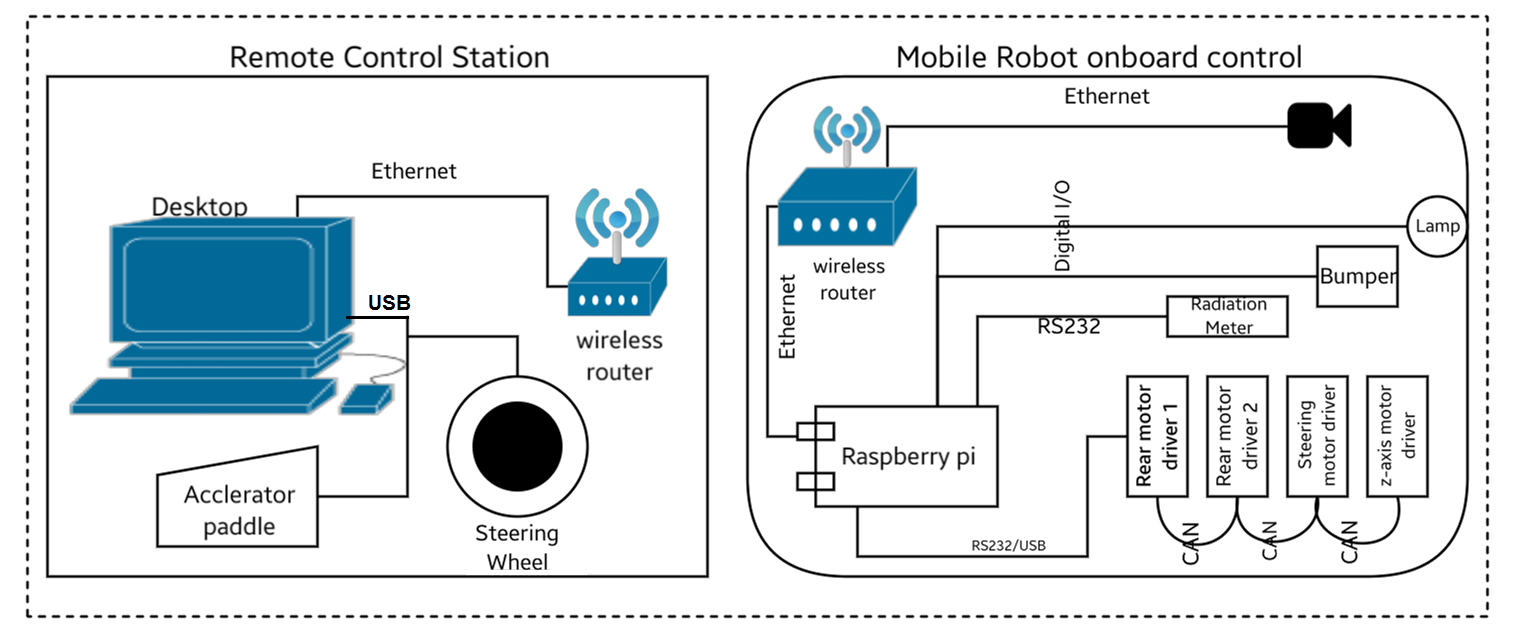
\includegraphics[width=\linewidth,keepaspectratio]{fig/controlblock}
		\captionof{figure}{Control architecture }
		\label{fig:ControlBlockDiag} 
	\end{figure}
	 The control station has a PC on which the video of  remote environment is displayed along with the vital statistics like current, speed, steer angle, platform height, battery status etc. of the mobile robot. Operator commands the robot by sending the steering angle and the speed by either using the joystick and paddle attached to the PC or using  keyboard. The exchange of data is at 20Hz. Raspberry Pi, the on-board controller of the robot first decodes the commands received, and based on the kinematic equation of the robot commands each of the motor.  The commands if fed directly to the motors after suitable kinematic transformations induces skidding of the robot during transient condition.  As the Ackerman condition shown in Figure \ref{fig:KenVec} is not satisfied during transient. This is due to difference in response time of the steering mechanism powered by the motor configured in position mode control, and the rear wheel motors which are configured in speed control mode.  This is very prominent in  case of step inputs. Therefore, the following algorithm was used.
	\begin{enumerate}
		\item Calculate the set point for steering motor $\theta_{SM} $ based on $\theta_s$. 
		\item Read the current steer  angle $\phi_{i}$.
		\item Calculate the rear wheel velocities set points $\omega_{i}$ and $\omega_{o}$ based on  $V$ and $\phi_{i}$.		
		\item Command  set points $\omega_{i}$, $\omega_{o}$ and $\theta_{SM} $ to each motor. 
	\end{enumerate} 
\begin{figure}[ht]
	\centering
	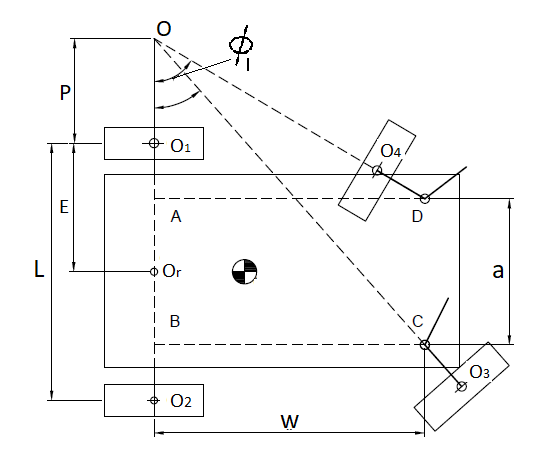
\includegraphics[width=4.5in]{fig/kinvec} 
	\caption{Ackerman steering condition}\label{fig:KenVec}
\end{figure}
Note that $\phi_{i}$ is the steer angle of the inner front wheel, V is the commanded linear velocity of point $O_r$ as shown in Figure \ref{fig:KenVec} and $\theta_s$ is the commanded steer angle. 


The on-board controller also calculates the current position of the robot based on wheel odometry. Different paths were traced and actual data collected to verify the accuracy of odometric results. It was observed that there is a lateral shift of 200 mm and a linear shift of 300 mm for 15000 mm long path. This clearly indicates slippage of wheels. 

\section{Simulation of Time Delay in Tele-operation}
 A functional relationship between mobility and latency in high-speed, teleoperated Unmanned Ground Vehicles under the context of path following has been presented in \cite{gorsich2018evaluating}. In this the  performance of  drivers were  evaluated under different time delays using a virtually simulated vehicle. 
 
 
The teleoperation  over wireless network for our system   resulted in delay of video feedback from robot camera. This is due to the large amount of data being transmitted. The delay was measured for the current system and it was found out to be around  
0.5sec, as shown in Figure \ref{fig:delayphoto}. The block digram shown in Figure \ref{fig:blockdigTimeDelay} depicts the architecture of the time delay system applicable to the current system. It may be noted that $T_2<<T_1$ for this system.
 \begin{figure}[ht]
 	\centering
 	\begin{minipage}{0.45\textwidth}
 		\centering
 		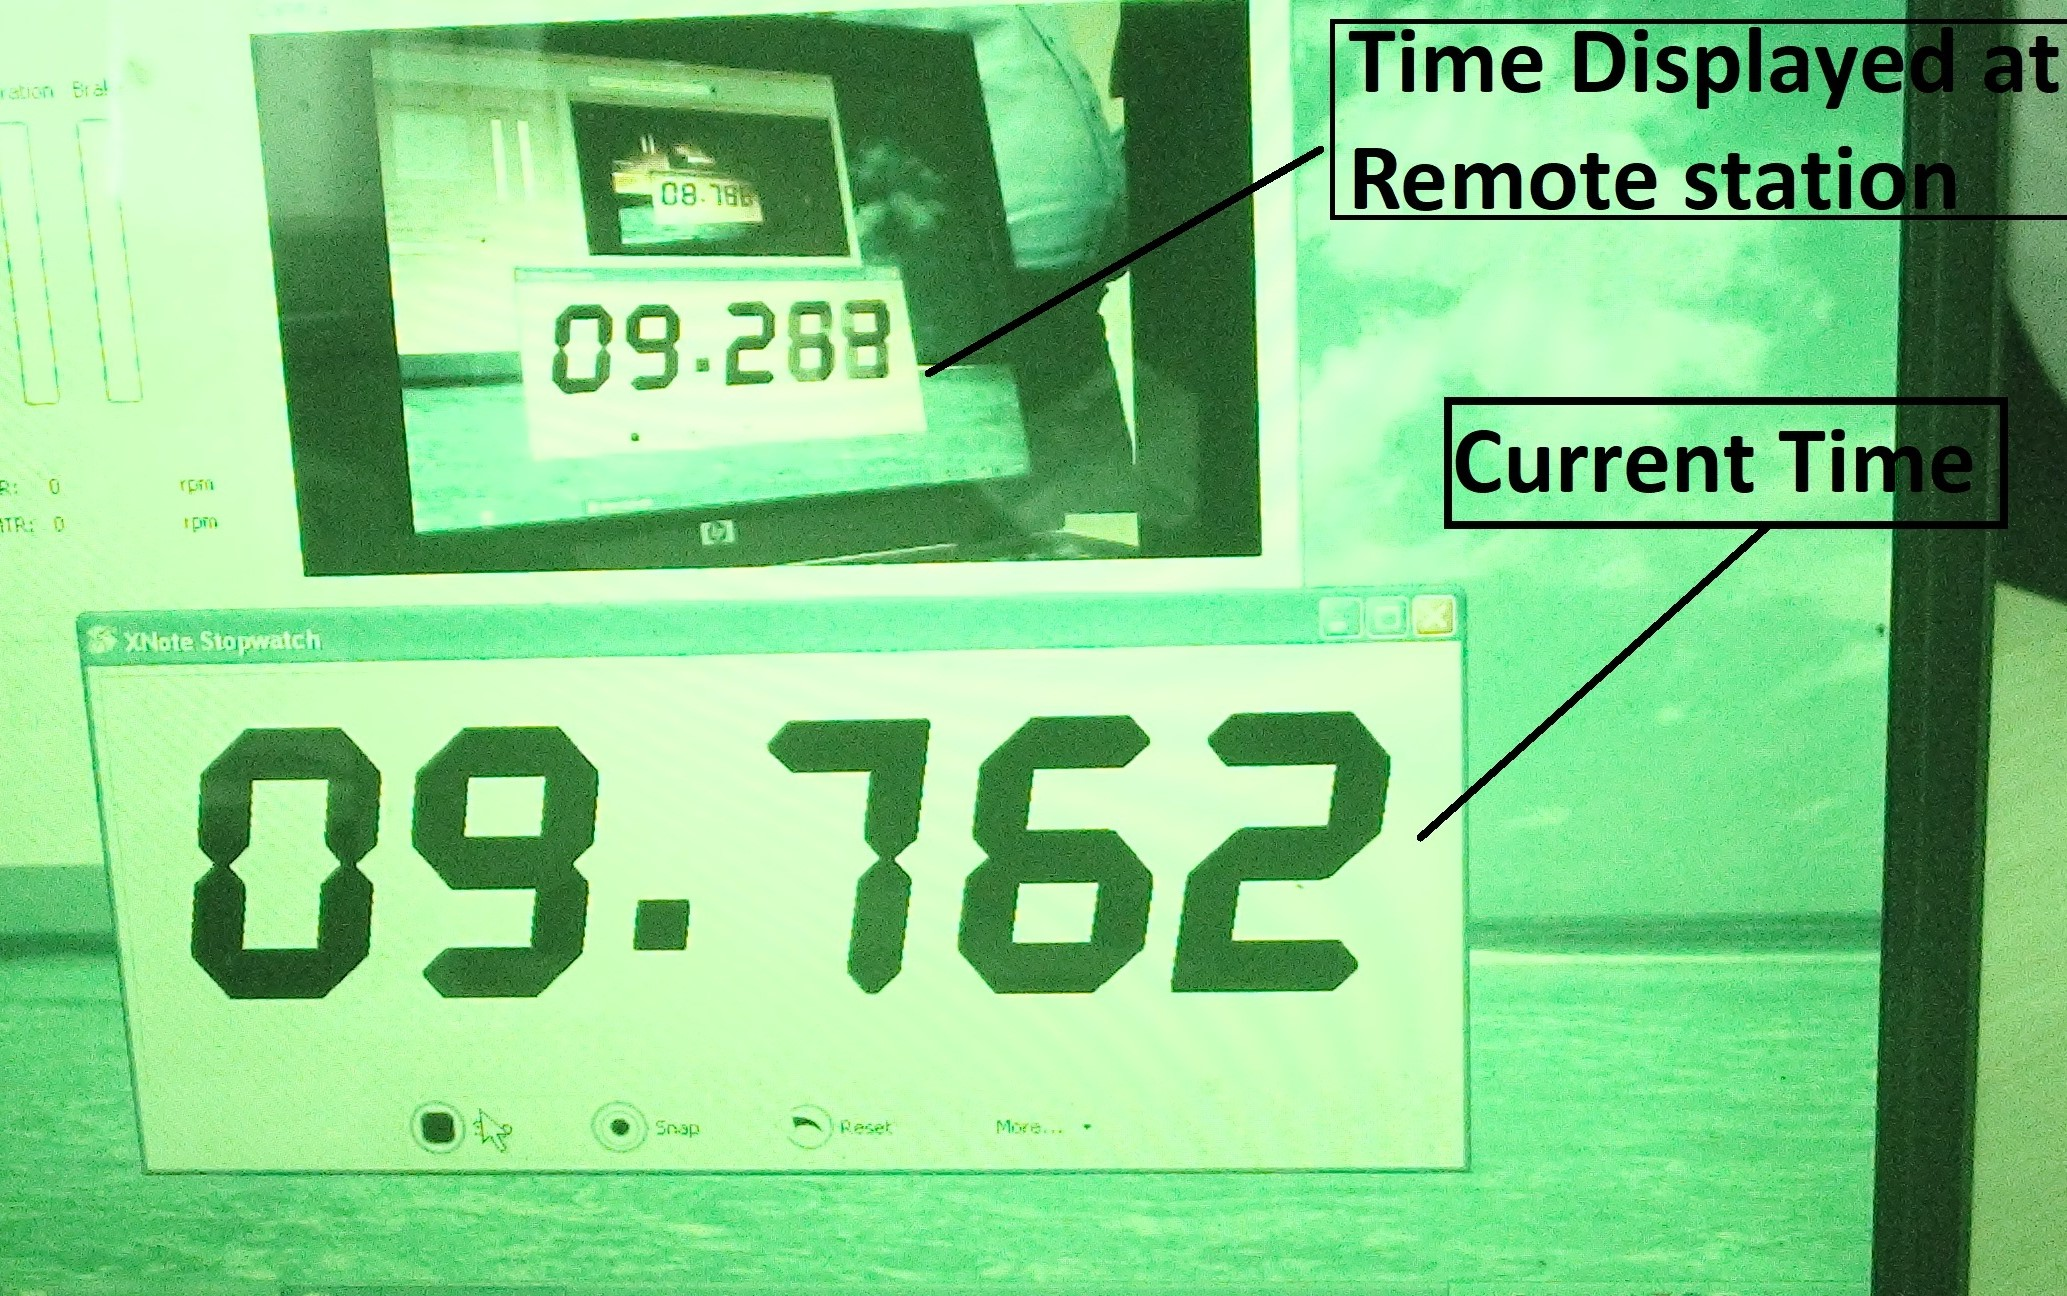
\includegraphics[width=\linewidth,keepaspectratio]{fig/delayMeasureNew}
 		\captionof{figure}{Delay measurment}
 		\label{fig:delayphoto}
 	\end{minipage}%
 	\begin{minipage}{0.55\textwidth}
 		\centering
 		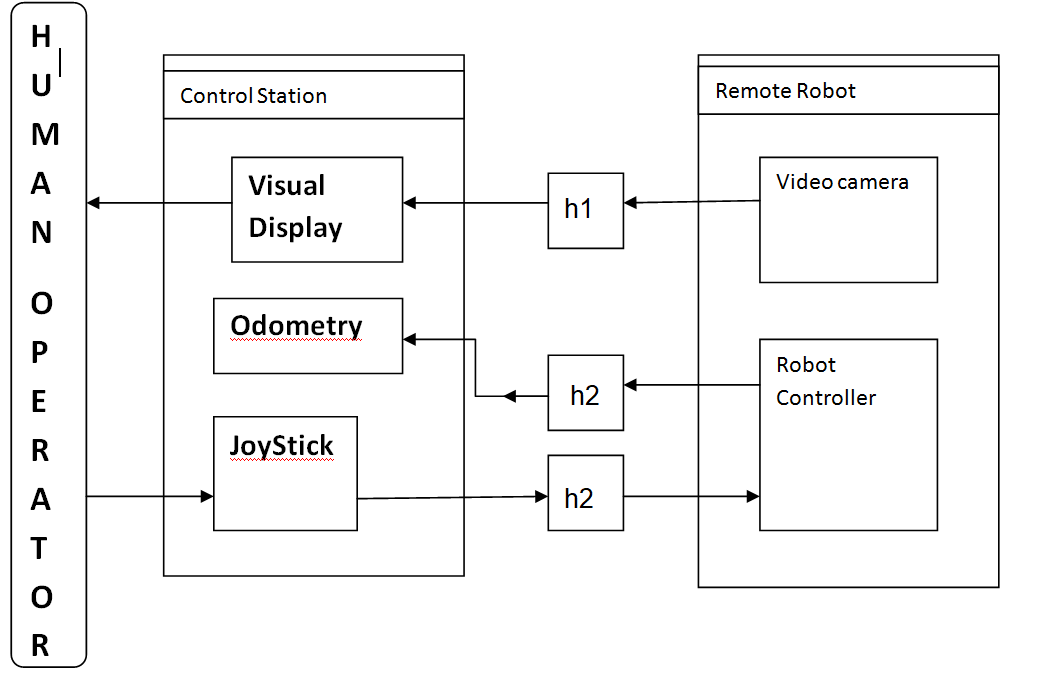
\includegraphics[width=.9\linewidth,keepaspectratio]{fig/BlockTimeDelay}
 		\captionof{figure}{Block digram of \\time delay system}
 		\label{fig:blockdigTimeDelay}
 	\end{minipage}
 \end{figure}
 In order to simulate and study the effect of time delay on the stability of the system, a mathematical model of the human operator's action has been proposed based on the pure pursuit algorithm proposed in \cite{coulter1992implementation}. It is assumed that the operator identifies a virtual path based on the obstacles, passageway and target location present in the visual image. He then targets a goal point on this virtual path and adjusts the steer angle of the vehicle towards it. This model of human operator was used in the simulation of teleoperation loop. The kinematic model of the mobile robot was used.  
 
 Stability of pure pursuit algorithm with input delay has been studied in \cite{ollero1995stability} and \cite{murphy1994analysis}. In both, the model was linearised and linear control  laws were used to predict stability. Since the vehicle and  human models are non linear, simulation was carried out to find the stability of the system under different time delays. It was found that the instability started at small time delay for short look ahead distance and higher vehicle velocity. The results are presented in Figure \ref{fig:delay500plot} and \ref{fig:delay800plot} for a circular path of $5m$ radius, look ahead distance of 0.5m and linear velocity of 0.5m/s.
\begin{figure}[ht]
\begin{minipage}{.5\textwidth}
	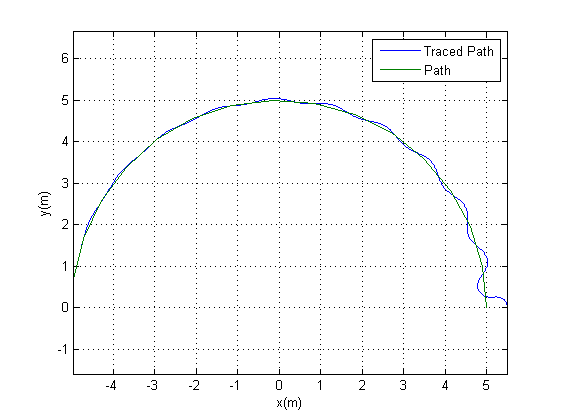
\includegraphics[width=\linewidth,keepaspectratio]{fig/Delay500milsec}
	\captionof{figure}{Simulation with time \\delay $h_1=.5sec$ and $h_2=0$ }
	\label{fig:delay500plot} 
\end{minipage} 
\hfill
\begin{minipage}{.5\textwidth}
	\centering
	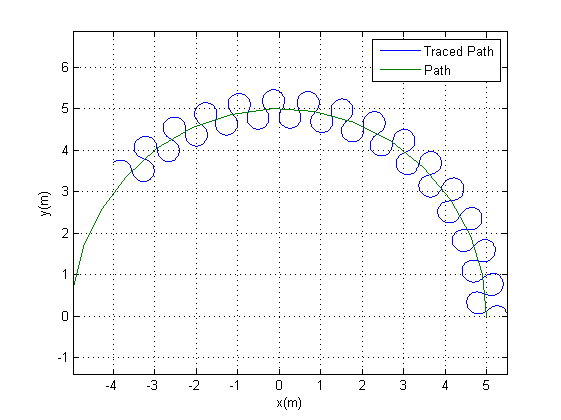
\includegraphics[width=\linewidth,keepaspectratio]{fig/Delay800milsec}
	\captionof{figure}{Simulation with  time \\delay $h_1=.8sec$ and $h_2=0$ }
	\label{fig:delay800plot} 
\end{minipage}
\end{figure}


To overcome the instability an approach based on Smith's predictor \cite{smith1959controller} was used. This was possible because the data exchange between the two stations was at 50ms loop, and was independent of the video feedback link, which had a typical delay of 500ms. A new pose was predicted based on the odometric data and fed to the "human operator model" for the intermediate control action. The simulation result presented in Figure \ref{fig:pred800plot} was obtained for 0.8s delay.  It is observed that the system is stable. This idea was used to modify the current teleoperation loop, as shown in Figure \ref{fig:predBlock}.  
 \begin{figure}[ht]
 	\begin{minipage}{.5\textwidth}
 		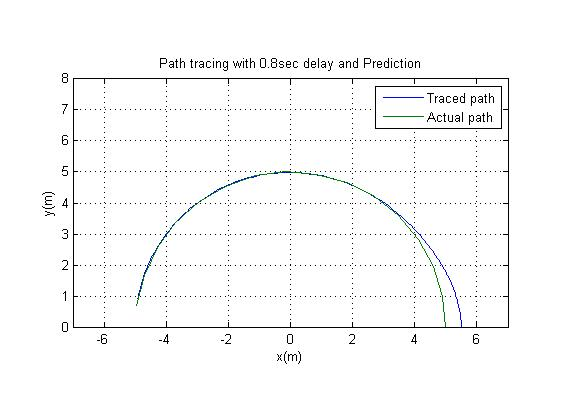
\includegraphics[width=\linewidth,keepaspectratio]{fig/withPrediction08delay}
 		\captionof{figure}{Simulation with  Predictor  \\ $h_1=.5sec$ and $h_2=0$ }
 		\label{fig:pred800plot} 
 	\end{minipage} 
 	\begin{minipage}{.5\textwidth}
 		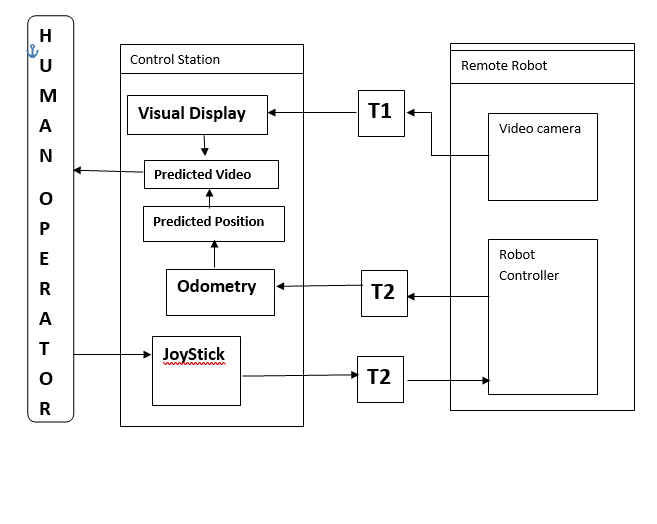
\includegraphics[width=\linewidth,keepaspectratio]{fig/PredictorBlockDig}
 		\captionof{figure}{Teleopration Loop with Predictor}
 		\label{fig:predBlock} 
 	\end{minipage}
 \end{figure}


\subsection{Predictive Display for  Teleoperation }
Psychophysics studies \cite{miall1993intermittency} and \cite{miall1985visuomotor} have shown short delay of 0.5 sec impairs the performance of an operate involved in teleoperation. Different factors affecting the teleoperation performance was discussed in \cite{chen2007human} in which time delay and depth perception was considered as major factors. One of the approaches to deal with the delay in visual feedback is predictive display presented in  \cite{deng2003predictive}, \cite{arai2016development} and \cite{bejczy1991role}. In \cite{deng2003predictive}, use of predictive display for  tele-operation of robotic arm in known environment using monocular camera mounted on robot arm helped them improve the operator performance. In \cite{arai2016development} predictive display was used for tele-opration of robot arm over internet.

In our present system,  RGB-D camera, namely  Kinect360 by Microsoft was used. The Kinect sensor provided synchronized RGB and depth data for each frame of the remote environment. The  color  and depth image of each frame was transformed to a common reference coordinate frame attached at point $O_r$ of the mobile robot shown in Figure \ref{fig:KenVec}. This gave the color and depth values of each pixel in the frame. A point cloud data (PCD) of the current view of the environment was generated using the camera model and the depth information of each pixel as shown in Figure \ref{fig:pcdt}.  
 \begin{figure}[ht]
	\begin{minipage}{.5\textwidth}
		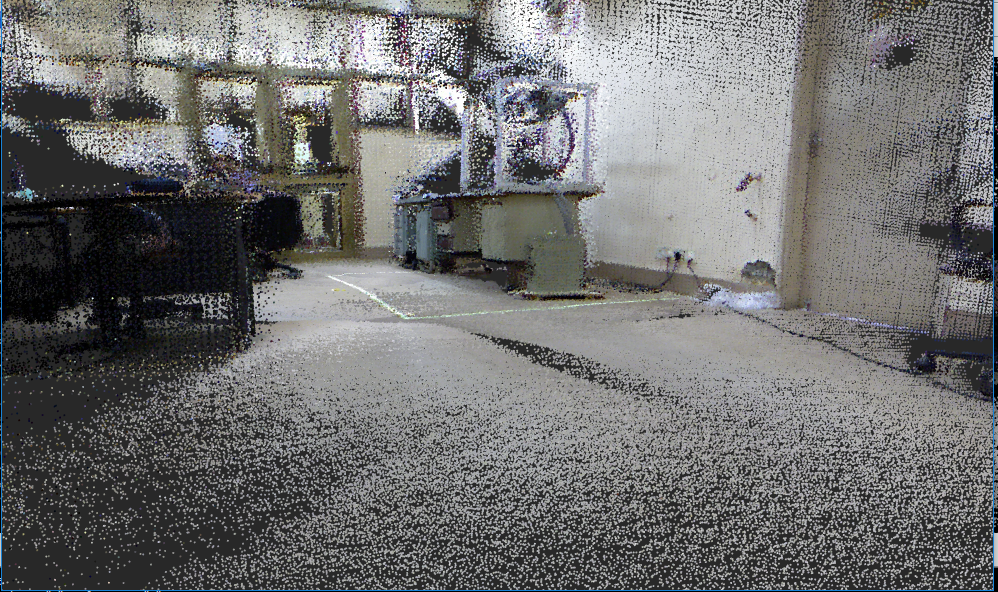
\includegraphics[height=4cm,keepaspectratio]{fig/pcdT}
		\captionof{figure}{PCD at time T }
		\label{fig:pcdt} 
	\end{minipage} 
	\begin{minipage}{.5\textwidth}
		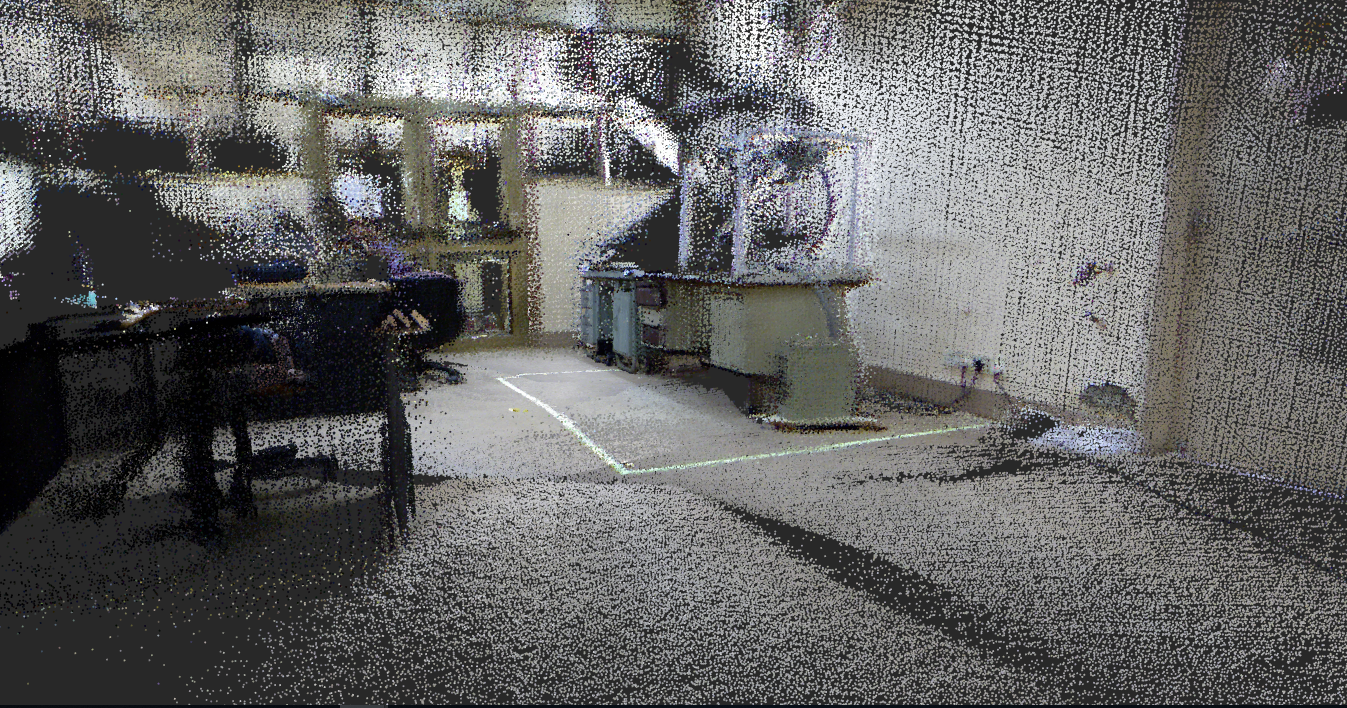
\includegraphics[height=4cm,,keepaspectratio]{fig/pcdT_p}
		\captionof{figure}{Predicted Scene}
		\label{fig:pcdP} 
	\end{minipage}
\end{figure}
 Due to the communication delay the view available at the control station as shown in Figure \ref{fig:pcdt} is $T_1$ sec old. 
 In other words, it is the view seen by the robot at time $t-T_1$, if $t$ is the current time. 
 The strategy followed here was not to present Figure \ref{fig:pcdt} to the operator but to present Figure \ref{fig:pcdP} which was generated from Figure \ref{fig:pcdt} by moving the view point $\Delta x, \Delta y$ and $\Delta \theta $, i.e, the value by which the robot might have changed its pose in time $T_1$.
  The change in pose was predicted by the kinematic model of the mobile robot and the control inputs.
   These data, as suggested earlier, has a much faster exchange loop of about 20Hz (50ms).  This method has greatly improved the driving capability of the operator in the presence of unavoidable time delay.
 
 \section{Conclusions}
 A customized mobile manipulator was designed for radiation measurement and mapping. The detail design aspects  based on the environment and mission requirement was discussed. The dynamic model of the system was also developed and simulation was carried out for specific path to verify the actuator requirements  and response time. A user interface and control architecture for teleoperation of this mobile manipulator was also discussed. The time delay introduced in video data transfer due to bandwidth limitation and image processing at camera end and its effect on system stability and poor operator performance  was also discussed. A predictive display of remote environment based on mathematical model of the mobile  robot was also presented. This strategy has largely  improved robot navigation by the operator even over delayed  communication network.  













	\bibliographystyle{ieeetr} %bibliography style-file
	\singlespacing
	
	\bibliography{zhref}
\end{document}